\documentclass [a4paper,12pt,oneside,final]{article}
\usepackage[left=15mm,top=15mm,right=15mm,bottom=20mm]{geometry}
\usepackage{tikz}
\usepackage{float}
\usetikzlibrary{arrows,positioning,shapes.geometric}

\title{%
Redes Neuronales \\
Análisis del modelo Integrate-and-Fire \\*[23pt]
Trabajo Práctico 2 \\
}
\date{2020}
\author{Igor Andruskiewitsch}

\begin{document}
    \maketitle

\section{Introducción}

\subsection{Modelo Integrate-and-Fire}

Este trabajo está orientado a comprender el modelo {\bf Integrate-and-Fire }, que modela la evolución temporal del potencial de membrana $ V_m(t) $ en el tiempo $ t $, entre el interior y el exterior de una neurona genérica. Descrito por la siguiente ecuación diferencial ordinaria (ODE):

\[ \dot{V_m}(t) = {1 \over \tau_m} (E_L - V_m(t) + R_m I_e(t)) \]

Donde:

\begin{itemize}
    \item {$ E_L $ es el potencial en reposo (mV) }
    \item {$ I_e(t) $ es la corriente eléctrica externa inyectada en el tiempo $ t $ (mV) }
    \item {$ R_m $ es la resistencia en megaOhms ($ M\Omega $) }
    \item {$ \tau_m $ es el tiempo característico de la membrana }
\end{itemize}

\section{Resolución Analítica}

\subsection{Pasos}

Si consideramos la corriente externa como una constante $ I_e(t) = I_e $, podemos buscar una solución analítica a nuestro modelo. Consideramos los siguientes valores para los parámetros:

\[ V_m(t = 0) = E_L = -65mV, \qquad R = 10 M \Omega, \]
\[ \qquad V_{th} = -50 mV, \qquad \tau_m = 10ms \qquad I_e = 2 nA \]

Comenzando con la resolución, teniendo en cuenta que ahora $ I_e $ es una constante, podemos reescribir la ecuación de la siguiente forma:

\[ \dot{V_m}(t) = {1 \over \tau_m} (E_L - V_m(t) + R_m I_e(t)) = A V_m(t) + B \]

Donde: $ \qquad A = { {- 1} \over \tau_m } \qquad B = { {R_m I_e + E_L} \over \tau_m } $


Comenzamos la resolución:

\[ V'(t) = A V(t) + B  \Rightarrow { V'(t) \over {A V(t) + B} } = 1 \]

Hacemos el reemplazo $ U(t) = A V(t) + B $, $ U'(t) = A V'(t) $, luego:

\[ V'(t) = { U'(t) \over A } \Rightarrow { U'(t) \over A U(t) } = 1 \Rightarrow { U'(t) \over U(t) } = A \Rightarrow { \int {U'(t) \over U(t)} dt } = \int { A dt } = A t + C \]

Ahora, sabiendo que $ \int { {f'(x) \over f(x)} dx } = \ln (f(x)) + C  $, vemos que:

\[ \ln (U(t)) = A t + C  \Rightarrow U(t) = e^{A t + C} = A V(t) + B \]
\[ \Rightarrow V(t) = {1 \over A} ( e^{At + C} - B ) = ({ e^C \over A }e^{At}) - { B \over A } \]

Tomando $ c^1 = { e^C \over A } $ y reemplazando $ A $ y $ B $ obtenemos:

\[ c^1 e^{-t \over \tau_m } - { {( R_m I_e + E_L ) \over \tau_m } \over {-1 \over \tau_m } } = c^1 e^{-t \over \tau_m } + R_m I_e + E_L \]

Ahora necesitamos conocer el valor de $ c^1 $. Esto lo podemos hacer ya que conocemos el valor inicial en $ t = 0 $:

\[ V_m(t = 0) = c^1 e^{ -t \over \tau_m } + R_m I_e + E_L = -65 \Rightarrow c^1 = - R_m I_e \]

Reemplazando, obtenemos:

\[ V_m(t) = (- R_m I_e) e^{-t \over \tau_m} + R_m I_e + E_L = (R_m I_e) (- e^{-t \over \tau_m} + 1) + E_L \]

Y observamos el siguiente gráfico al graficar la fórmula encontrada para $ 0ms \leq t \leq 200ms $:

\begin{figure}[ht]
  \centering
  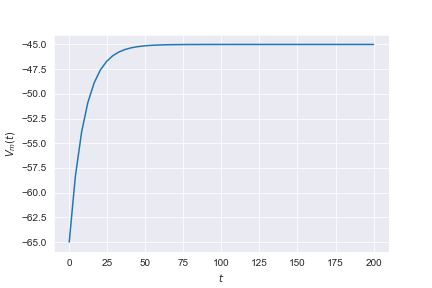
\includegraphics[width=10cm,keepaspectratio]{./diagramas/grafico_a.png}
  \caption{Gráfico de la solución analítica sin umbral de disparo}
\end{figure}

\pagebreak
\subsection{Comparación con RK4}

En esta sección, vamos a comparar los resultados dados por la resolución analítica sin considerar el umbral de disparo, con los resultados dados por la aproximación usando RK4 (incluyendo el umbral de disparo). Ambos se realizan utilizando $ 0ms \leq t \leq 200ms $ y el caso de RK4 con un paso de integración $ h = 0.05 $.

\begin{figure}[ht]
  \centering
  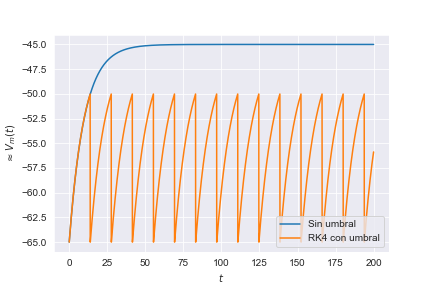
\includegraphics[width=10cm,keepaspectratio]{./diagramas/grafico_b.png}
  \caption{Comparación entre solución analítica sin umbral de disparo y aproximación con RK4 con umbral de disparo en $-50$}
\end{figure}

Podemos observar que ambos métodos comienzan con una crecida exponencial y mientras que uno se estabiliza, el otro vuelve a realizar el mismo proceso ya que vuelve al valor inicial. Esto se debe a que en el primer gráfico no incluimos el {\it umbral de disparo}. 

\section{Comprensión de $I_e$}

En esta sección vamos a realizar algunos experimentos para comprender la importancia del {\bf input} $I_e$ en el modelo. Vamos a comenzar por intentar entender la relación entre $I_e$ y la frecuencia del disparo variando con $ 0 \leq I_e \leq 50  $:

\begin{figure}[ht]
  \centering
  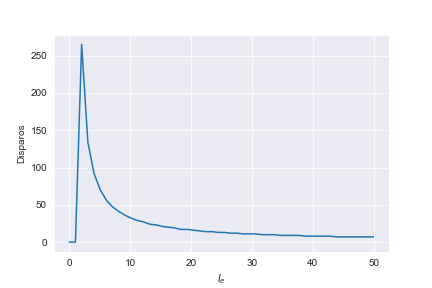
\includegraphics[width=11cm,keepaspectratio]{./diagramas/grafico_c.png}
  \caption{Relación entre $I_e$ y la frecuencia de disparo}\label{fig:c}
\end{figure}

Como podemos observar en la figura \ref{fig:c}, para los casos $I_e = 0$ y $I_e = 1$ no hay ningún disparo y por lo tanto su frecuencia es 0. Sin embargo, para $I_e = 2$ ya obtenemos disparos y a medida que $I_e$ incrementa tenemos una frecuencia cada vez más baja (y por lo tanto más disparos). Si bien no vamos a buscar cuál es la relación exacta entre estos valores, podemos observar fácilmente que parece ser de la forma $e^{-x}$ con una traslación. Esta observación es interesante, ya que la resolución analítica que obtuvimos anteriormente era de la forma $e^x$.

\subsection{Variando $I_e$ de manera uniforme}

Al comienzo habíamos definido el $I_e(t)$ como una función que depende de $t$, luego, para poder encontrar una solución analítica pasamos a tomar $I_e(t) = I_e$ como una constante. Ahora vamos a variar a $I_e$ de manera uniforme entre $0$ y $5$ para cada $t$, para ver cómo se comporta el modelo:

\begin{figure}[ht]
  \centering
  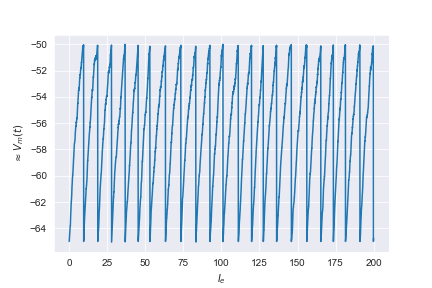
\includegraphics[width=11cm,keepaspectratio]{./diagramas/grafico_d.png}
  \caption{Aproximación del modelo con $I_e$ uniformemente distribuido}\label{fig:d}
\end{figure}

En la figura \ref{fig:d} podemos observar que aún variando uniformemente el valor de $I_e$ en función de $t$, seguimos viendo {\it picos}, y a una frecuencia similar a la que obtuvimos con $I_e = 2$ (un poco más baja). También observamos que las curvas de crecimiento del modelo ya no son de la forma $e^x$ ya que encontramos variaciones que reflejan el flujo discontinuo de entrada.

\section{Conclusión}


\end{document}
